% !TEX root = Thesis.tex
% Change "draft" to "final" when you're done.
\documentclass[12pt,letterpaper,oneside,notitlepage]{report}

\usepackage[top=1in,left=1.5in,right=1in,bottom=1in]{geometry}

\usepackage{fontspec,lipsum}
\usepackage{mathpazo}
\defaultfontfeatures{Ligatures=TeX}
\usepackage[small,sf,bf]{titlesec}

%\usepackage{xltxtra}
%\usepackage{xunicode}

%\usepackage{subcaption}
\usepackage{graphicx}
\usepackage{rotating}

\usepackage{todo}

\graphicspath{{images/}}

\usepackage{setspace}
\doublespacing

\usepackage{titling}

\usepackage{unicode-math}
\usepackage{amsmath}
\usepackage{amsthm}

\usepackage{algorithm}
\usepackage{algorithmic}

%\usepackage{tikz}

\usepackage{minted}

%\usemintedstyle{bw}

\usepackage{booktabs}

\usepackage{nag}

\usepackage{upquote}

\usepackage[backend=biber]{biblatex}
\addbibresource{Thesis.bib}

%\input tikz
%\usetikzlibrary{fit}

%\usemintedstyle{default}

\setmainfont[
	Numbers=OldStyle,
	Kerning=Uppercase,
	% Not allowed to use any fonts > 10pt.
	%SizeFeatures={
	%	{Size={6-10}, Font=* Caption},
	%	{Size={10.01-}, Font=*}
	%}
	]{Garamond Premier Pro}
\setsansfont{Futura Std}
\setmathfont{STIXGeneral}
%\setmonofont{Anonymous Pro}
\setmonofont{Consolas}

\newmintedfile[cljcode]{clj}{linenos,frame=topline,frame=lines,framesep=2mm}

\renewcommand{\theFancyVerbLine}{\ttfamily{\scriptsize {\arabic{FancyVerbLine}}}}

\newcommand{\thesistitle}[8]{
	\title{#1}
	\author{#2}

	\begin{titlepage}
		\centering
		\vspace{2cm}
			{\huge\sc #1}\\[1cm]

			by\\[1cm]

			{\Large #2}\\[2cm]

			\singlespacing{A Thesis Submitted in Partial Fulfillment\\of the Requirements for the Degree of}\\[1cm]

			#3\\[0.5cm]

			in\\[0.5cm]

			Faculty of #4\\[0.5cm]

			#5\\[1.5cm]

			University of Ontario Institute of Technology\\[1.5cm]

			Supervisor:  #6\\[1.5cm]

			#7 #8\\[3cm]

			Copyright \copyright\ #2 #8
	\end{titlepage}}

\theoremstyle{definition}
\newtheorem{defn}{Definition}

\begin{document}
	\pagenumbering{roman}
	
	\thesistitle{The Chronicles of Molly}{Richard J.I. Drake}{Master of Science (MSc)}{Science}{Computer Science}{Dr. Ken Q. Pu}{August}{2013}
	
	%\thispagestyle{empty}
	%\clearpage
	
	%\pagenumbering{roman}
	\setcounter{page}{3}

	\begin{abstract}
		Traditional relational database systems offer powerful data modelling and querying capabilities.  Unfortunately a relational database does not permit users to perform natural (keyword) queries.  We present a system for automatic mapping of a relational schema into a document schema in order to facilitate fast and powerful full-text (keyword) search.  By providing a facility for users to conduct keyword searches, we improve accessibility and decrease search time complexity.  In addition, we explore further improvements to time complexity by utilizing concurrent implementations of our search algorithms.
		
		\textbf{Keywords} relational database; full-text search
	\end{abstract}

%	\begin{acknowledgements}
%		\lipsum[2]
%	\end{acknowledgements}

	\chapter*{Preface}
		\section*{Background and Motivation}
			The introduction of keyword search has revolutionized how we find information.  Over the years, numerous techniques have been developed which make searching through large amounts of information for one or more keywords extremely fast.  With the advent of faster computer hardware, we are able to not only search through small attributes of a document (eg. Title, synopsis, etc.) but rather the entirety of the document itself.
		
			An example of an early system which utilized keyword search would be a library catalogue.  Such a system would allow a user to search, by keyword, for the title of a book, manuscript, etc.  The results would show item titles matching the keyword(s), as well as other information such as whether or not the item is in circulation, as well as where it is located within the library.  This information would come from a relational database.
		
			With the rise of the World Wide Web, much information was placed online.  This information would be easy to access if one knew how to locate it.  Unfortunately, over time, so much information existed on the World Wide Web that it became difficult to keep track of it all.  There was a need to index all of this information and make it accessible.  This need was filled by a Web search engine.
		
			Initial Web search engines comprised of simple scripts that gathered listings of files on FTP servers; they were essentially link farms.  A few short years later, the first full-text (keyword) search engine, WebCrawler, was released.
		
			While full-text search engines provided an excellent means for locating information, as the Web grew larger, the volume of noise also grew larger.  In addition, every Web page could be structured in a different way; the Web was largely a collection of unstructured documents.  That is, there were few obvious links between them.
		
			Search engines such as Google attempted to solve this problem by introducing new algorithms, such as PageRank, to rank Web pages on both the relevance of their content as well as their reputation.  The idea was if a page is linked to often, it is considered to be more authoritative on a subject than a page with fewer links.  This allowed the relevance of a page to be computed based on not only its contents, but its artificial importance.
		
			Molly attempts to avoid some of the issues plaguing search engines.  It deals primarily with structured, filtered data.  This allows us to provide results with less noise.  In addition, the fact that it deals with structured data means links between documents are explicitly stated.  Rather than inferring a link between documents based on hyperlinks, we know when two documents are linked together.
		
			This thesis provides an overview of the Molly system.
		
		\section*{Outline}
			Changed.

	\tableofcontents

	\listoftables
	\listoffigures
	\listofalgorithms

	\clearpage
	\pagenumbering{arabic}
	
	\chapter{Definitions}
		\section{Data Representation \& Notation}
		\label{sec:data-representation-notation}
			The data from the database is represented in various data structures.  There are separate representations for each type of data:  values, entities, and entity groups.

				\subsubsection{Value}
					\begin{defn}
						A \textbf{Value} represents a single piece of information.  To avoid repetition, each value is unique.  That is, $\exists! v \in V$, where $v$ is a value in the set $V$ of all values.
					\end{defn}

				\subsubsection{Entity}
					\begin{defn}
						An \textbf{Entity} is a collection of attributes, $a_n$, each mapped to a single value, $v_n$.  An entity also includes additional information such as a unique identifier.

						\begin{figure}[!ht]
							\centering
							\[
								\begin{array}{ll}
									\mathrm{id} & T_n|v_{id} \\
									a_1 & v_1 \\
									a_2 & v_2 \\
									\vdots & \vdots \\
									a_n & v_n
								\end{array}
							\]
							\caption{The structure of an entity}
							\label{fig:entity-rep}
						\end{figure}

						Entities are analogous to rows in a database table.  Thus, the unique identifier is generated based on the table name, $T_n$, as well as unique key in the table, $v_{id}$.  The unique key identifies the row, and the table name identifies the table.  Together they uniquely identify the entity within the entire database.  Attributes are analogous to columns in a database table.

						$\exists! e_{id} \in E$, where $E$ is the set of all entities.
					\end{defn}

				\subsubsection{Entity Group}
					\begin{defn}
						An \textbf{Entity Group} joins together two or more entities.  These entity groups can also have attributes, $a_n$, and values, $v_n$, associated with them much like entities.

						\begin{figure}[!ht]
							\centering
							\[
								\begin{array}{ll}
									e_L & \left[ e_1, e_2, \ldots, e_n \right] \\
									a_1 & v_1 \\
									a_2 & v_2 \\
									\vdots & \vdots \\
									a_n & v_n
								\end{array}
							\]
							\caption{The structure of an entity group}
							\label{fig:entity-group-rep}
						\end{figure}

%						\begin{tikzpicture}[auto=left,every node/.style={circle}]
%							\node (e1) at (1,1) {$e_1$};
%							\node (e2) at (4,1)  {$e_2$};
%							\node (e3) at (7,1)  {$e_3$};
%							\node (e4) at (10,1) {$e_4$};
%							\node (e5) at (13,1)  {$e_5$};
%
%							\foreach \from/\to in {e1/e2,e2/e3,e3/e4,e4/e5}
%								\draw (\from) -- (\to);
%							
%							\node (rect) [draw,dotted,fit=(e1) (e2) (e3)] {};
%							\node[draw,dotted,fit=(e3) (e4) (e5)] {};
%
%						\end{tikzpicture}
					\end{defn}

	\chapter{RDBMS to Document Store}
		\begin{figure}[ht!]
			\cljcode[firstnumber=9,firstline=9,lastline=11]{../src/molly/datatypes/entity.clj}
			\caption{Determining whether or not a field is classified as ``special.''}
			\label{src:molly-datatypes-entity-special}
		\end{figure}
		
		\begin{figure}[ht!]
			\cljcode[firstnumber=13,firstline=13,lastline=28]{../src/molly/datatypes/entity.clj}
			\caption{Unique identifier generation.}
			\label{src:molly-datatypes-entity-uid}
		\end{figure}
		
		\begin{figure}[ht!]
			\cljcode[firstnumber=30,firstline=30,lastline=35]{../src/molly/datatypes/entity.clj}
			\caption{Creation of a field.}
			\label{src:molly-datatypes-entity-field}
		\end{figure}
		
		\begin{figure}[ht!]
			\cljcode[firstnumber=37,firstline=37,lastline=43]{../src/molly/datatypes/entity.clj}
			\caption{Creation of a document.}
			\label{src:molly-datatypes-entity-document}
		\end{figure}
		
		\begin{figure}[ht!]
			\cljcode[firstnumber=45,firstline=45,lastline=75]{../src/molly/datatypes/entity.clj}
			\caption{Transformation of a row into the internal representation.}
			\label{src:molly-datatypes-entity-row-data}
		\end{figure}
		
		\begin{figure}[ht!]
			\cljcode[firstnumber=77,firstline=77,lastline=90]{../src/molly/datatypes/entity.clj}
			\caption{Transformation of a document into the internal representation.}
			\label{src:molly-datatypes-entity-doc-data}
		\end{figure}
		
		\begin{figure}[ht!]
			\cljcode[firstnumber=92,firstline=92,lastline=114]{../src/molly/datatypes/entity.clj}
			\caption{Transformation of the internal representation into a document.}
			\label{src:molly-datatypes-entity-data-doc}
		\end{figure}
	
	\chapter{Concurrency}
		\begin{figure}[ht!]
			\cljcode[firstnumber=6,firstline=6,lastline=10]{../src/molly/algo/common.clj}
			
			\caption{Retrieves the entity with the given ID.}
			\label{src:molly-algo-common-find-entity-by-id}
		\end{figure}
		
		\begin{figure}[ht!]
			\cljcode[firstnumber=12,firstline=12,lastline=19]{../src/molly/algo/common.clj}
			
			\caption{Finds all groups containing an entity with the given ID.}
			\label{src:molly-algo-common-find-group-for-id}
		\end{figure}
		
		\begin{figure}[ht!]
			\cljcode[firstnumber=21,firstline=21,lastline=23]{../src/molly/algo/common.clj}
			
			\caption{Finds adjacent nodes in the graph (entities linked in groups).}
			\label{src:molly-algo-common-find-adj}
		\end{figure}
		
		\begin{figure}[ht!]
			\cljcode[firstnumber=4,firstline=4,lastline=19]{../src/molly/algo/bfs.clj}
			
			\caption{Discovers new nodes along the frontier and updates the state accordingly.}
			\label{src:molly-algo-bfs-update-adj}
		\end{figure}
		
		\begin{figure}[ht!]
			\cljcode[firstnumber=21,firstline=21,lastline=34]{../src/molly/algo/bfs.clj}
			
			\caption{BFS using recursion.}
			\label{src:molly-algo-bfs-bfs}
		\end{figure}
		
		\begin{figure}[ht!]
			\cljcode[firstnumber=4,firstline=4,lastline=13]{../src/molly/algo/bfs_atom.clj}
			
			\caption{Discovers new nodes along the frontier and updates the state accordingly.}
			\label{src:molly-algo-bfs-atom-update-adj}
		\end{figure}
		
		\begin{figure}[ht!]
			\cljcode[firstnumber=15,firstline=15,lastline=26]{../src/molly/algo/bfs_atom.clj}
			
			\caption{Implements a concurrent version of BFS using atoms.}
			\label{src:molly-algo-bfs-atom-bfs-atom}
		\end{figure}
		
		\begin{figure}[ht!]
			\cljcode[firstnumber=4,firstline=4,lastline=16]{../src/molly/algo/bfs_ref.clj}
			
			\caption{Discovers new nodes along the frontier and updates the state accordingly.}
			\label{src:molly-algo-bfs-ref-update-adj}
		\end{figure}
		
		\begin{figure}[ht!]
			\cljcode[firstnumber=18,firstline=18,lastline=29]{../src/molly/algo/bfs_ref.clj}
			
			\caption{Implements a concurrent version of BFS using references.}
			\label{src:molly-algo-bfs-ref-bfs-atom}
		\end{figure}
	
	\chapter{Theoretical}
		The problem of efficiently searching through a graph is the subject of countless articles and journal papers.  Numerous algorithms have been proposed to perform graph search in an efficient manner.  Many of these algorithms build upon their predecessors, making assumptions and changing aspects to better suit a particular problem area.
		
		The applications of efficient graph search algorithms are endless.  Algorithms such as Dijkstra's are used heavily in path finding, for example in a portable GPS unit.  A* Search is used in the area of computer vision to approximate the best path to take.  Companies such as Amazon make use of graph search algorithms in order to find related products for consumers to purchase.
		
		This thesis concentrates on building a system which can be utilized in order to discover related information.  The system that was built is capable of finding not only related information from neighbouring nodes, but also the best path between two arbitrary nodes.
		
		Section \ref{sec:data-rep-and-notation} provides an overview of how the data is represented in the system.  It also defines notation to represent this data.  Section \ref{sec:database-abstraction} outlines how the relational database is related to the data in the system.  Section \ref{sec:data-corpus} provides an example data corpus which is utilized throughout this thesis.  It details the ``mycampus'' dataset.  Finally, Section \ref{sec:graph-search-algos} provides justification for the algorithm chosen to perform the graph search.  It discusses multiple different graph search algorithms, as well as why the one used in this thesis was chosen.
		
		\section{Data Representation \& Notation}
		\label{sec:data-rep-and-notation}
			The data from the database is represented in various data structures.  There are separate representations for each type of data:  values, entities, and entity groups.

				\subsubsection{Value}
					\begin{defn}
						A \textbf{Value} represents a single piece of information.  To avoid repetition, each value is unique.  That is, $\exists! v \in V$, where $v$ is a value in the set $V$ of all values.
					\end{defn}

				\subsubsection{Entity}
					\begin{defn}
						An \textbf{Entity} is a collection of attributes, $a_n$, each mapped to a single value, $v_n$.  An entity also includes additional information such as a unique identifier.

						\begin{figure}[!ht]
							\centering
							\[
								\begin{array}{ll}
									\mathrm{id} & T_n|v_{id} \\
									a_1 & v_1 \\
									a_2 & v_2 \\
									\vdots & \vdots \\
									a_n & v_n
								\end{array}
							\]
							\caption{The structure of an entity}
							\label{fig:entity-rep}
						\end{figure}

						Entities are analogous to rows in a database table.  Thus, the unique identifier is generated based on the table name, $T_n$, as well as unique key in the table, $v_{id}$.  The unique key identifies the row, and the table name identifies the table.  Together they uniquely identify the entity within the entire database.  Attributes are analogous to columns in a database table.

						$\exists! e_{id} \in E$, where $E$ is the set of all entities.
					\end{defn}

				\subsubsection{Entity Group}
					\begin{defn}
						An \textbf{Entity Group} joins together two or more entities.  These entity groups can also have attributes, $a_n$, and values, $v_n$, associated with them much like entities.

						\begin{figure}[!ht]
							\centering
							\[
								\begin{array}{ll}
									e_L & \left[ e_1, e_2, \ldots, e_n \right] \\
									a_1 & v_1 \\
									a_2 & v_2 \\
									\vdots & \vdots \\
									a_n & v_n
								\end{array}
							\]
							\caption{The structure of an entity group}
							\label{fig:entity-group-rep}
						\end{figure}

%						\begin{tikzpicture}[auto=left,every node/.style={circle}]
%							\node (e1) at (1,1) {$e_1$};
%							\node (e2) at (4,1)  {$e_2$};
%							\node (e3) at (7,1)  {$e_3$};
%							\node (e4) at (10,1) {$e_4$};
%							\node (e5) at (13,1)  {$e_5$};
%
%							\foreach \from/\to in {e1/e2,e2/e3,e3/e4,e4/e5}
%								\draw (\from) -- (\to);
%							
%							\node (rect) [draw,dotted,fit=(e1) (e2) (e3)] {};
%							\node[draw,dotted,fit=(e3) (e4) (e5)] {};
%
%						\end{tikzpicture}
					\end{defn}
					
		\section{Relational Database Abstraction}
		\label{sec:database-abstraction}
		
		\section{Data Corpus}
		\label{sec:data-corpus}
			For illustrative purposes, the mycampus dataset will be used.  This data comes from UOIT's course registration system.
			% TODO:  Fix footnotes.
			% \footnote{http://uoit.ca/mycampus/}.
			
			There are several different entities which comprise the mycampus dataset:
			
			\begin{itemize}
				\item Courses
				\item Instructors
				\item Schedules
				\item Sections
				\item Teaches
			\end{itemize}
			
			The \textbf{Courses} entity represents a course.  A course has an individual code, along with a title and a description (See Table  \ref{tbl:courses-entity-schema}).  The code uniquely identifies the course.
			
			\begin{table}[!htp]
				\centering
				\begin{tabular}{lll}
					\toprule
					Column & Type & Description \\
					\midrule
					code & VARCHAR & Unique course code \\
					title & VARCHAR & Title of the course \\
					description & TEXT & A brief description \\
					\bottomrule
				\end{tabular}
				\caption{Courses entity schema}
				\label{tbl:courses-entity-schema}
			\end{table}
			
			The \textbf{Instructors} entity represents an individual instructor.  Each instructor has a unique identifier, as well as a name (See Table \ref{tbl:instructors-entity-schema}).  An instructor can be a Professor, Lecturer, Sessional Instructor, or Teaching Assistant.
			
			\begin{table}[!htp]
				\centering
				\begin{tabular}{lll}
					\toprule
					Column & Type & Description \\
					\midrule
					id & INT & Unique identifier \\
					name & VARCHAR & The instructor's name \\
					\bottomrule
				\end{tabular}
				\caption{Instructors entity schema}
				\label{tbl:instructors-entity-schema}
			\end{table}
			
			The \textbf{Sections} entity represents a section of a course.  Courses may have many sections.  For example, one section could be a lecture, while another is a lab.  Some courses may have over a dozen sections, depending on the associated term.
			
			Each section contains a unique identifier, capacity information (students enrolled, spots open, etc.), when registration is open for the section, how many credits it is worth, what level (eg. undergraduate or graduate), and what year the section is offered in (See Table \ref{tbl:sections-entity-schema}).
			
			\begin{table}[!htp]
				\centering
				\begin{tabular}{lll}
					\toprule
					Column & Type & Description \\
					\midrule
					id & INT & Unique identifier \\
					actual & INT & Number of people enrolled in the course \\
					campus & VARCHAR & String uniquely identifying the campus \\
					capacity & INT & Maximum number of people that may be enrolled in the section \\
					credits & FLOAT & Number of credits awarded upon successful completion \\
					levels & VARCHAR & The level of the course (eg. undergraduate, graduate, etc.) \\
					registration\_start & DATE & Date registration for the section opens \\
					registration\_end & DATE & Date registration for the section ends \\
					semester & VARCHAR & String that uniquely identifies the semester \\
					sec\_code & INT & Unique section code (called a CRN) \\
					sec\_number & INT & Sequential number identifying the number of the section \\
					year & INT & The year the section is offered in \\
					\bottomrule
				\end{tabular}
				\caption{Sections entity schema}
				\label{tbl:sections-entity-schema}
			\end{table}
			
			The \textbf{Schedules} entity represents a scheduled meeting of a section.  A section may have many schedules.  For example, a lecture section may meet twice a week.
			
			Each schedule has a unique identifier, a date range in which the schedule is active, the time of the schedule, the type, location, and the day which the class takes place (See Table \ref{tbl:schedules-entity-schema}).
			
			\begin{table}[!htp]
				\centering
				\begin{tabular}{lll}
					\toprule
					Column & Type & Description \\
					\midrule
					id & INT & Unique identifier \\
					date\_start & DATE & First day of class \\
					date\_end & DATE & Last day of class \\
					day & VARCHAR & Single character representing the day of the week \\
					schedtype & VARCHAR & Lecture, tutorial, lab, etc. \\
					hour\_start & INT & Hour the class starts at \\
					hour\_end & INT & Hour the class ends at \\
					min\_start & INT & Minute the class starts at \\
					min\_end & INT & Minute the class ends at \\
					classtype & VARCHAR & The type of class \\
					location & VARCHAR & Unique location name where class is held \\
					\bottomrule
				\end{tabular}
				\caption{Schedules entity schema}
				\label{tbl:schedules-entity-schema}
			\end{table}
			
			A \textbf{Teaches} entity is used to link together an instructor and a schedule.  Each link has a unique identifier along with the instructor's position (eg. Teaching Assistant, Lecturer, etc.) (See Table \ref{tbl:teaches-entity-schema}).
			
			\begin{table}[!htp]
				\centering
				\begin{tabular}{lll}
					\toprule
					Column & Type & Description \\
					\midrule
					id & INT & Unique identifier \\
					position & VARCHAR & Position of the Instructor with regard to a Schedule \\
					\bottomrule
				\end{tabular}
				\caption{Teaches entity schema}
				\label{tbl:teaches-entity-schema}
			\end{table}
		
		\section{Graph Search Algorithms}
		\label{sec:graph-search-algos}
			Careful consideration was given to which graph search algorithm was to be used.  Among the choices were:
			
			\begin{itemize}
				\item Breadth-First
				\item Bellman-Ford
				\item Dijkstra
				\item A*
			\end{itemize}
			
			The first choice, Breadth-First Search, is among the simplest of the algorithms.  It has the advantage of being simple to implement.  It can only handle fixed costs for travelling between nodes, which can be a disadvantage.
			
			Bellman-Ford is similar to BFS.  It has the ability to deal with variable cost.  This comes at the cost of increased difficulty in implementation.  When the cost between nodes is fixed, Bellman-Ford essentially becomes BFS.
			
			A greedy version of BFS is Dijkstra's Algorithm.  It utilizes a priority queue rather than a regular queue, allowing it to be faster.  As it is a greedy algorithm, Dijkstra's Algorithm may not return the optimal result.
			
			An extension to Dijkstra's is A* search.  Graph search spaces can be rather large.  A* attempts to prune the search space based on a heuristic.  A* is a natural choice to perform graph search in certain areas such as computer vision where an obvious heuristic exists.  It has a disadvantage of consuming large amounts of memory (though IDA* attempts to limit memory consumption).
			
			There are many more graph search algorithms.  The above were primarily considered as many of the other algorithms are simple extensions with different data structures.
			
			For this application, there is no obvious heuristic.  This eliminates A*.  There is also no obvious cost function.  This eliminates Dijkstra's Algorithm.  Bellman-Ford is very similar to BFS with the added ability to deal with variable cost.  As the cost function is not obvious and thus constant, Bellman-Ford essentially reverts back to BFS.
			
			For these reasons, BFS was chosen as the graph search algorithm.  While the other candidates and others provide numerous advantages over BFS in many situations, this is not one of them.
	
	\chapter{Implementation}
		\section{Functional vs. Procedural Programming of Algorithms}
			Functional and procedural programming languages are entirely different paradigms.	In functional programming, data is immutable.  Functions must be pure and predictable (free of ``side effects'').  Loops and control flow are accomplished with recursion and pattern matching.
			
			Procedural languages allow for more flexibility at a cost of unpredictability.  
			
			Key differences between FP and procedural (for algorithms)
			
			\subsection{Functional Data Structures}
				Clojure immutable data structures, versioning (persistent data structures), STM vs. locking
			
		\section{Tuneable Parameters}
			Tuneable parameters
	
	\chapter{System Implementation}
		\section{Technology Selection}
			
			
			\subsection{Programming Language}
				Numerous programming languages were considered for the implementation.  Among them were:  Ruby, Python, and Clojure.  Each of the languages presented both pros and cons.  Ruby and Python are rather similar object oriented languages.  Clojure is a functional language.
				
				Ruby features a clean syntax and is very object oriented.  Its object model was inspired by that of Smalltalk.  It has a very active web development community and numerous web frameworks (eg. Rails, Sinatra, Padrino, etc.).  In contrast to Python, it features a lean core, instead choosing to depend on third party libraries.
				
				Python also features clean syntax and is object oriented.  It embraces a ``batteries included'' philosophy to its standard library, featuring libraries for everything from serial communications to importing/exporting CSV files.  It too has a strong web development community and numerous web frameworks (eg. Django, Flask, web2py, etc.).
				
				Python is used extensively by scientists.  As such, it has numerous plotting, computation, and simulation libraries.  Examples include Matplotlib, SciPy, NumPy, and NetworkX.
				
				Both of the above languages embrace functional programming elements.  Python has filter, reduce, and map.  Ruby's collections are also capable of performing filter (select), reduce (inject), and map.  They both lack an important aspect of functional programming:  immutable objects.
				
				Clojure is a purely functional language built on top of the JVM.  Like Python and Ruby, it is dynamically typed.  Unlike Python and Ruby, it is a Lisp dialect and as such features macros and code-as-data.
				
				As it runs on the JVM, Clojure allows us to utilize existing Java languages.  Using Java libraries through Python or Ruby requires using their respective native code interfaces to Java's JNI.  This process is typically automated through a tool such as SWIG.
				
				Clojure was chosen as the implementation language for a number of reasons.  First of all, as it is built on top of the JVM, it can utilize JDBC for database access.  It can also make use of several other useful libraries.  Secondly, its dynamic Lisp nature is a natural way of processing data.  Clojure allows us to model our data structures directly after the data.  In a language such as Python, one would need to make use of classes.
			
			\subsection{Relational Database}
				Several relational database management engines (RDBMS) were evaluated for this project.  Key requirements were SQL support, and JDBC driver availability.
				
				SQL, or Structured Query Language, is a powerful way to make complex queries.  It is loosely based on Relational Algebra (RA)\cite[p.~243]{dbsys-06}.  In addition to being a data-manipulation language (similar to Relational Algebra), it is also a data-definition language.
				
				JDBC, or Java Database Connectivity, was required in order for our application to access the database.  JDBC is an API which allows us to access a database using a standard interface.  It is the responsibility of the JDBC Driver to translate the API calls into the correct syntax for the database engine.
				
				Any RDBMS that supports SQL-92 or higher and has a JDBC driver for it should be usable in this system.  For testing purposes, we chose to use SQLite.  SQLite provided a SQL interface, had a stable JDBC driver, and is ubiquitous.  SQLite is an embedded database, allowing for local development without running a separate daemon process.
			
			\subsection{Full-Text Search Database}
				Two full-featured full-text search databases (FTSDB) were evaluated.  The first, Xapian, is written as a C++ library.  It features a rich query language, high performance, and a scalable design\cite{xapian}.  Bindings for Java are made available via a simple JNI library.
				%\footnote{http://xapian.org/docs/bindings/java/README}
				
				The second, Lucene, is a pure-Java library.  It too features a rich query language and reasonable performance.  Lucene also forms the basis of the Apache Solr search platform.  As it is written in Java, Lucene runs natively on the JVM.
				
				Both choices provided plenty of features, Java interfaces, and excellent performance.  Ultimately Lucene was chosen.  As it ran on the JVM, interfacing with the Lucene library from our Clojure code was simple.  The fact that it was written in pure-Java and required no native libraries meant the entire project could be bundled as a Java Archive (JAR).
			
			\subsection{Web Stack}
				Clojure is a young language.  As such, few web frameworks exist specifically for it (it can, however, interface with any Java web framework).  
				
				Clojure web frameworks are built on top of Ring, itself an HTTP abstraction layer with adapters for Java servlets as well as the Jetty web server.  Ring is similar to WSGI in Python, or Rack in Ruby.
				
				The web framework chosen for this project was Noir.  Noir provided a simple Clojure API for building the JSON API to allow for client-side querying of the project's API.
			
		\section{System Design}
			The system is split into numerous components.
			
			A configuration file is used to describe the entities and entity groups.  It defines the relationship between entities, as well as their attributes and values.  This configuration file is used by the crawler and indexer in order to retrieve data from the relational database and index it in a full-text search database.
			
			Once the index is built, another component provides an internal API for querying the full-text search database.  It is a thin Clojure wrapper over the Lucene API which provides the basis for search and retrieval of results.  This wrapper is utilized by the system to discover relationships among entities.
			
			Finally, the system can be interfaced with via a JSON API.  The JSON API provides a simple HTTP wrapper around the search and discovery features of the system.  The use of JSON allows client-side JavaScript to send and receive queries with XMLHttpRequest.
			
			\todo{Add overview diagram of system design.}
			
			\subsection{Configuration}
				Configuration files are simply Clojure code that follow a well-defined protocol.  The protocol defines three main components of the system:
				
				\begin{itemize}
					\item[\texttt{connection}] The relational database connection.  It must be an instance of the \texttt{Database} protocol.
					\item[\texttt{index}] The path to the full-text search database index file.
					\item[\texttt{schema}] A definition of the database schema.  The definition includes both the definition of entities, as well as the definition of entity groups.  The schema is a list of instances of the \texttt{Schema} protocol.
				\end{itemize}
				
				\subsubsection{\texttt{Database} Protocol}
					The \texttt{Database} protocol is defined as follows.
					
					\begin{minted}{clj}
(defprotocol Database
	(execute-query [this query f]))
					\end{minted}
					
					Each database instance must provide a function which accepts a query and function as arguments.  It must execute the query provided and call function \texttt{f} on each row returned.
				
				\subsubsection{\texttt{Schema} Protocol}
					The \texttt{Schema} protocol is defined as follows.
					
					\begin{minted}{clj}
(defprotocol Schema
  (crawl [this db-conn idx-w])
  (klass [this])
  (schema-map [this]))
  				\end{minted}
					
					A schema consists of the following information:
					
					\begin{itemize}
						\item A symbol (typically the name of the table).
						\item A hash map containing the structure of the schema.
					\end{itemize}
					
					Schemas are also responsible for populating the full-text search index with data from the relational database.
					
					A concrete implementation for this protocol is provided by the \texttt{EntitySchema} type.
		
		\section{Implementation Issues}
	
	\chapter{Performance \& Evaluation}
		\section{Environment}
			All benchmarks were run on the same machine using the same software versions.  The machine has the following specs.
			
			\begin{table}[!ht]
				\centering
				\begin{tabular}{ll}
					\toprule
					Item & Description \\
					\midrule
					Model & Dell PowerEdge 2950 \\
					Processor & 2 x Quad-Core Intel\textregistered\ Xeon\texttrademark\ 5300 3.0GHz \\
					Memory & 8 GB DDR2 ECC RAM 667 MHz \\
					\bottomrule
				\end{tabular}
			\end{table}
			
			Along with the following software versions.
			
			\begin{table}[!ht]
				\centering
				\begin{tabular}{ll}
					\toprule
					Item & Description \\
					\midrule
					Operating System & GNU/Linux Ubuntu 10.04.4 LTS \\
					Kernel & 2.6.32-28-generic \\
					Java\texttrademark\ SE Runtime Environment & 1.6.0\_26-b03 \\
					Java HotSpot\texttrademark\ 64-Bit Server VM & 20.1\-b02 \\
					\bottomrule
				\end{tabular}
			\end{table}
		
		\section{Methodology}
			Evaluating the performance of code is a difficult problem at best.  It is difficult to determine the impact on performance of various uncontrollable factors.  Virtual Machines add another layer of abstraction which introduces even more factors.
			
			As this project runs a top of the Java Virtual Machine (JVM), there are many factors to consider with regard to performance.  In addition to uncontrollable events such as garbage collection, the JVM's behaviour can differ based on the operating system (OS) it is running on.
			
			\subsection{Pitfalls of the Java Virtual Machine}
				Reliable benchmarking on the JVM is a difficult problem.  The standard HotSpot VM utilizes a non-deterministic garbage collector (GC).  In addition, the JIT is also non-deterministic.  These two problems combine into a larger issue.
				
				\subsubsection{Timing Execution}
					There are two methods provided by the JVM for getting a precise time from the OS; \\\texttt{System.currentTimeMillis()} and \texttt{System.nanoTime()}.  The former returns the ``wall'' time.  It is possible for time to leap forward or backward using this method.  If daylight savings time occurs between calls to \texttt{System.currentTimeMillis()}, it can result in a negative time.
					
					The latter uses a variety of methods in order to obtain the precise time.  The method it uses depends on both the OS and the hardware itself.  Under Windows, \texttt{System.nanoTime()} makes use of the \texttt{QueryPerformanceCounter(QPC)} call.  This call may make use of the ``programmable-interval-timer (PIT), or the ACPI power management timer (PMT), or the CPU-level timestamp-counter (TSC).'' \cite{hotspot-timer-06}  Accessing the PIT and PMT is a slow operation.  Accessing the TSC is a very fast operation, but may result in varying numbers \cite{linux-tsc-06}.
					
					Linux attempts to use the TSC when possible.  If it finds the values to be unreliable (eg. different cores vary too much), it makes use of the High Precision Event Timer (HPET) \cite{linux-tsc-06}.
					
					\begin{table}[!ht]
						\centering
						\begin{tabular}{lc}
							\toprule
							Platform & Resolution (ms) \\
							\midrule
							Windows 95/98 & 55 \\
							Windows NT, 2000, XP (single processor) & 10 \\
							Windows XP (multi processor) & 15.625 \\
							Linux 2.4 Kernel & 10 \\
							Linux 2.6 Kernel & 1 \\
							\bottomrule
						\end{tabular}
						\caption{Reported resolutions of \texttt{currentTimeMillis()} by platform \cite{rob-java-bench-08}.}
					\end{table}
					
					The JVM's timing functions are one area where the JVM's behaviour differs based on the OS.  Different operating systems provide varying degrees of time resolution.  The speed at which the OS-level calls to these timing functions return can even differ.
				
				\subsubsection{Garbage Collection}
			
				\subsubsection{Just-in-Time Compilation}
					A typical JVM only loads classes when they're first used \cite{rob-java-bench-08}.  This task typically involves disk I/O, along with extra processing.  As a result, the initial run of a task may only...
			
			\subsection{Mitigating JVM Pitfalls}
				\subsubsection{JIT Compilation}
					\begin{figure}[ht!]
						\cljcode[firstnumber=33,firstline=33,lastline=41]{../src/molly/core.clj}
			
						\caption{core.clj}
					\end{figure}
		
		\begin{figure}[!ht]
			\centering
			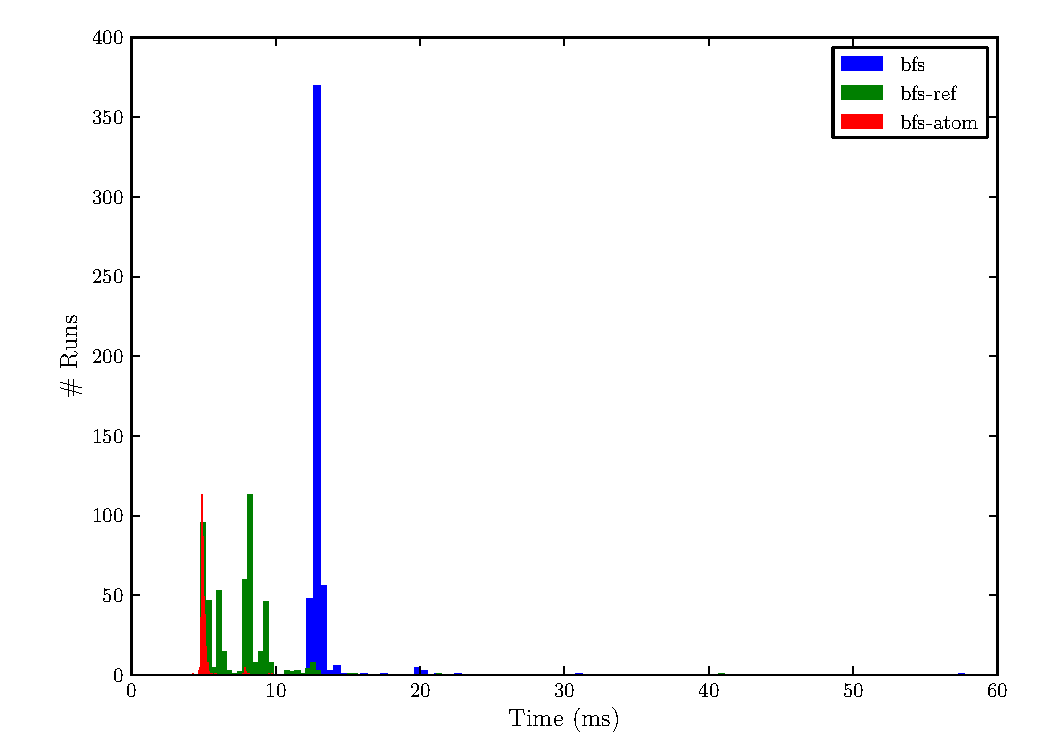
\includegraphics[scale=0.85]{1_hops}
			\caption{1 Hop}
			\label{fig:perf-1-hop}
		\end{figure}
		
		\begin{figure}[!ht]
			\centering
			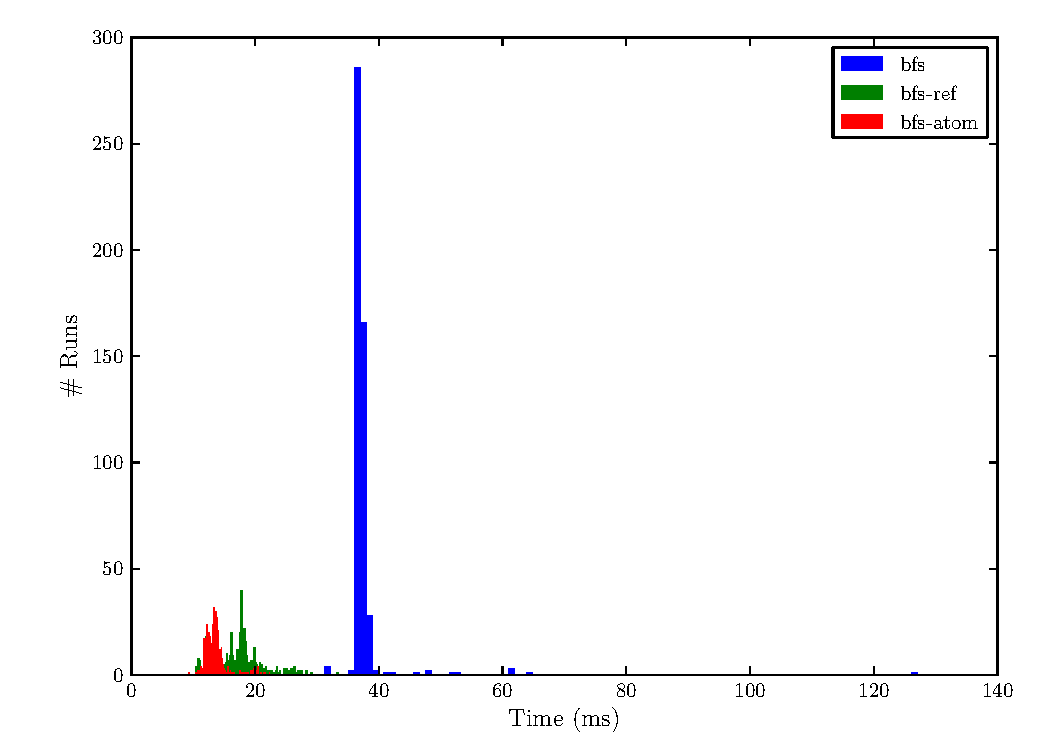
\includegraphics[scale=0.85]{2_hops}
			\caption{2 Hops}
			\label{fig:perf-2-hops}
		\end{figure}
		
		\begin{figure}[!ht]
			\centering
			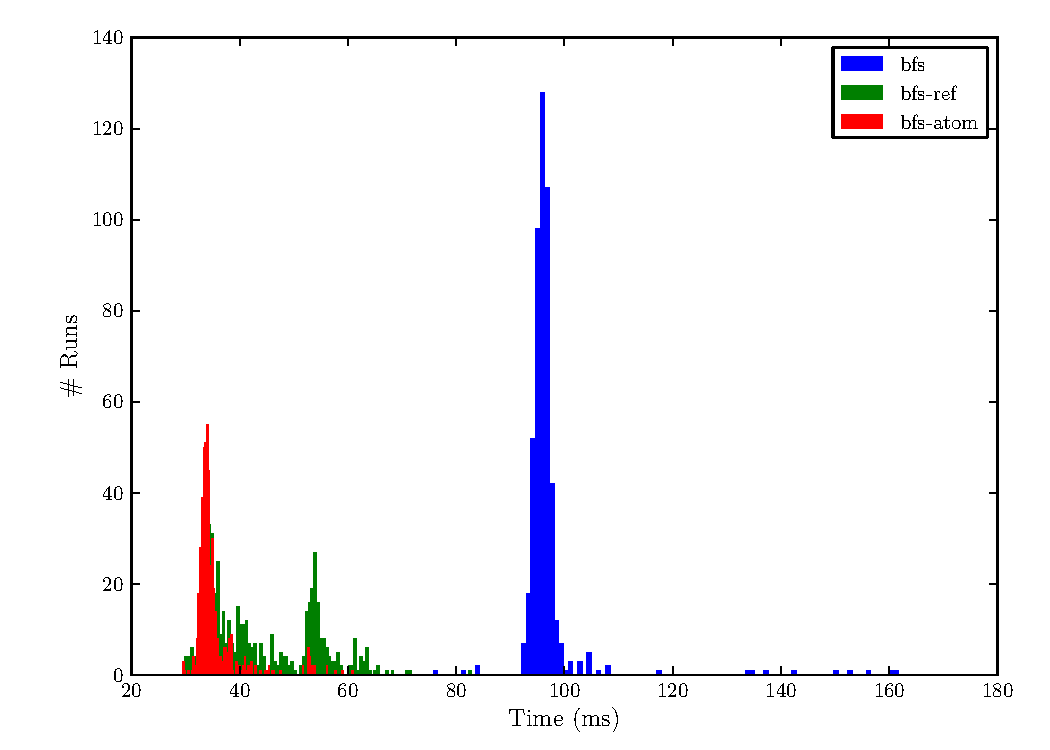
\includegraphics[scale=0.85]{3_hops}
			\caption{3 Hops}
			\label{fig:perf-3-hops}
		\end{figure}
		
		\begin{figure}[!ht]
			\centering
			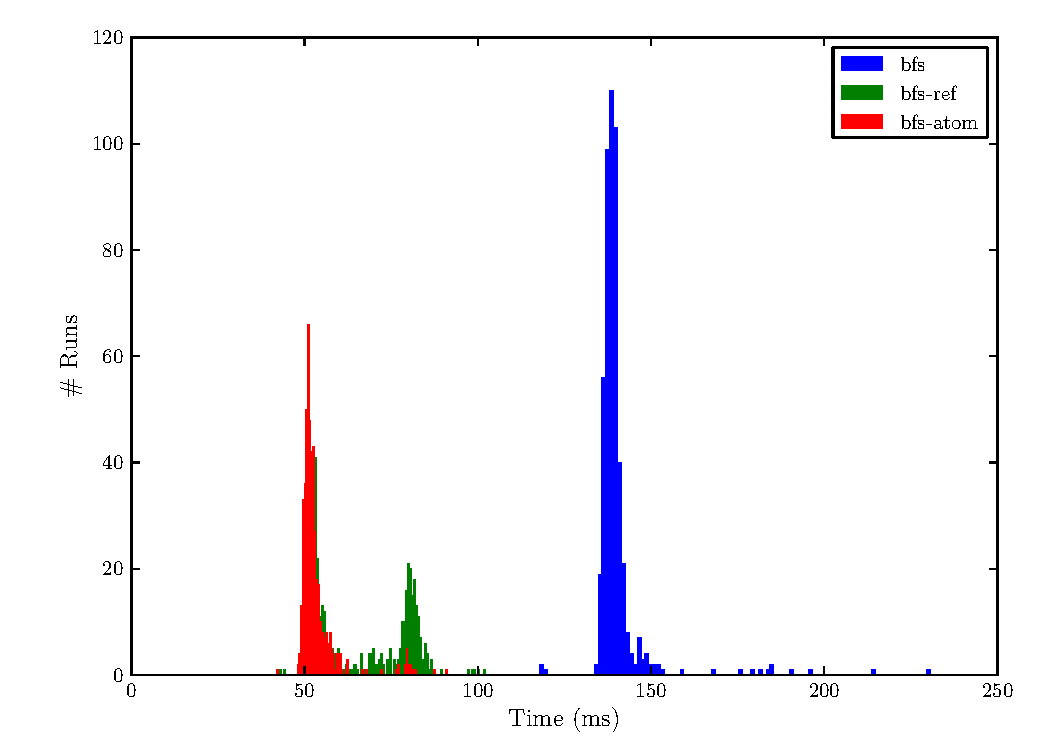
\includegraphics[scale=0.85]{4_hops}
			\caption{4 Hops}
			\label{fig:perf-4-hops}
		\end{figure}
		
		\begin{figure}[!ht]
			\centering
			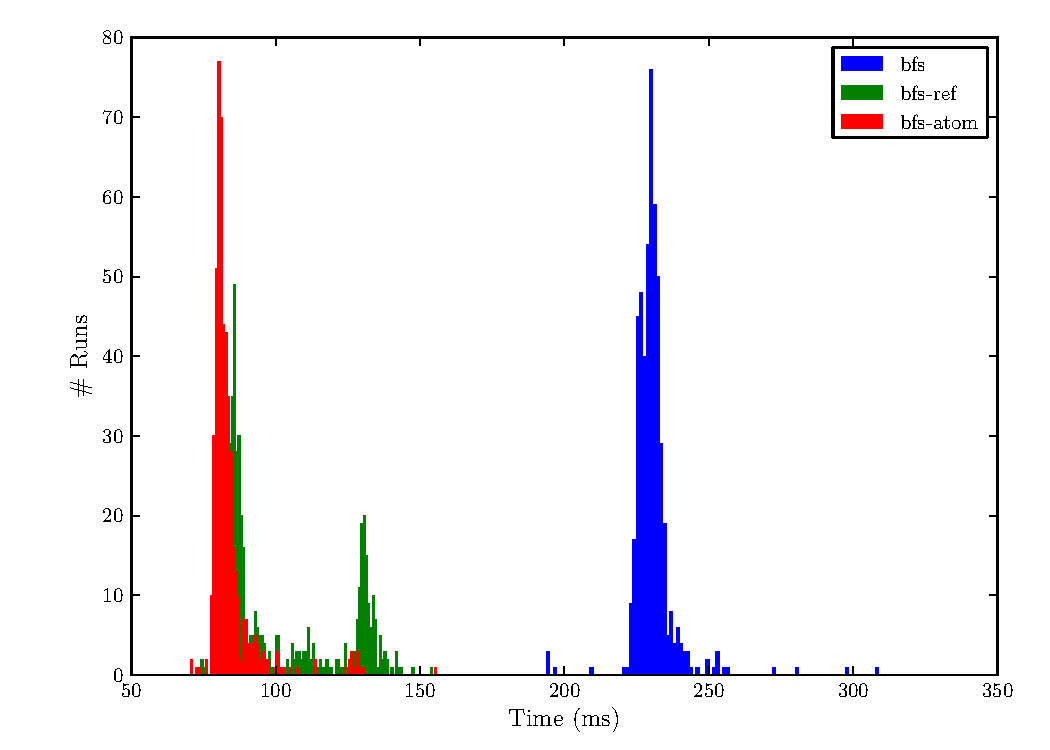
\includegraphics[scale=0.85]{5_hops}
			\caption{5 Hops}
			\label{fig:perf-5-hops}
		\end{figure}
		
		\begin{figure}[!ht]
			\centering
			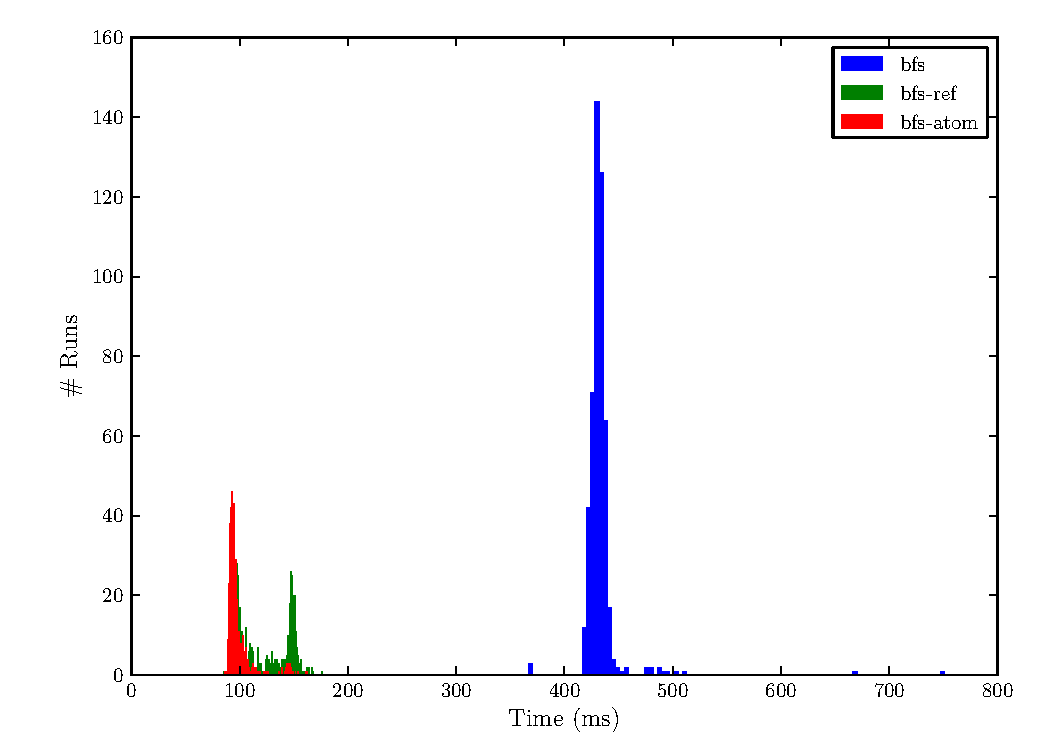
\includegraphics[scale=0.85]{6_hops}
			\caption{6 Hops}
			\label{fig:perf-6-hops}
		\end{figure}
		
		\begin{figure}[!ht]
			\centering
			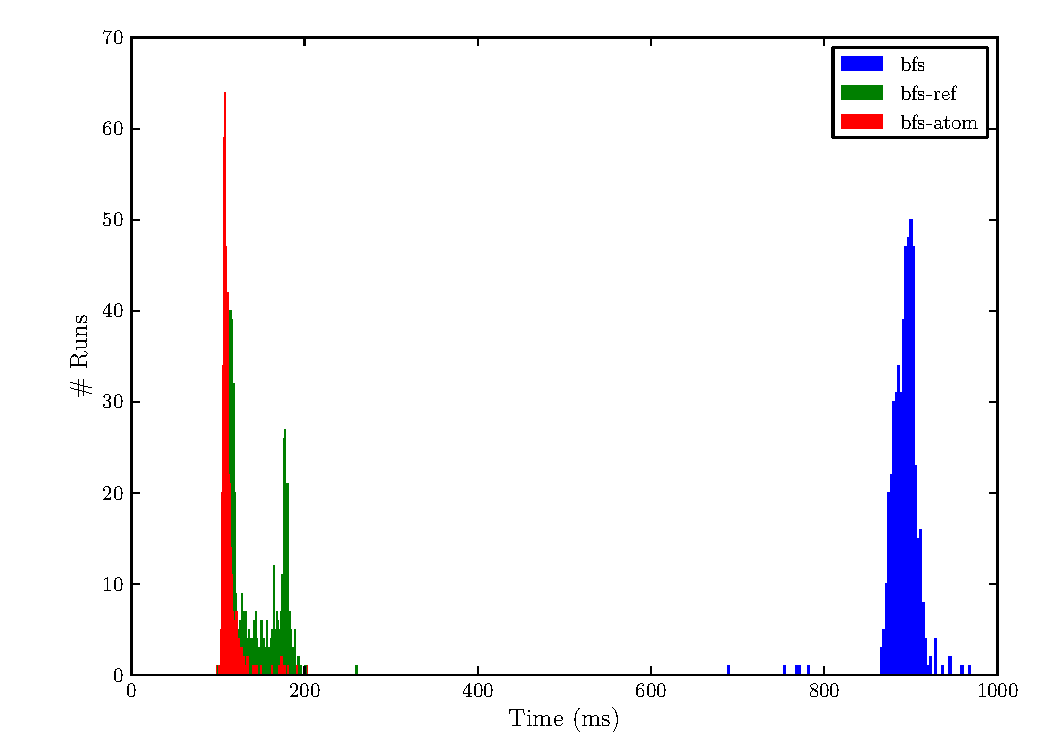
\includegraphics[scale=0.85]{7_hops}
			\caption{7 Hops}
			\label{fig:perf-7-hops}
		\end{figure}
		
		\begin{figure}[!ht]
			\centering
			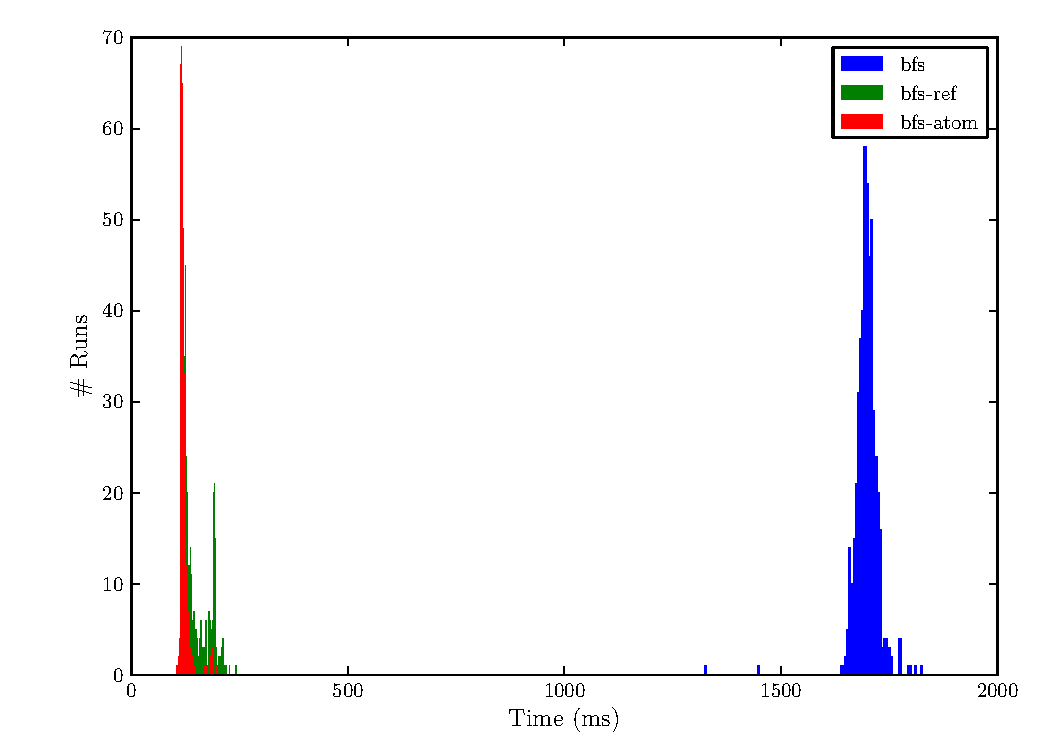
\includegraphics[scale=0.85]{8_hops}
			\caption{8 Hops}
			\label{fig:perf-8-hops}
		\end{figure}
		
		\begin{figure}[!ht]
			\centering
			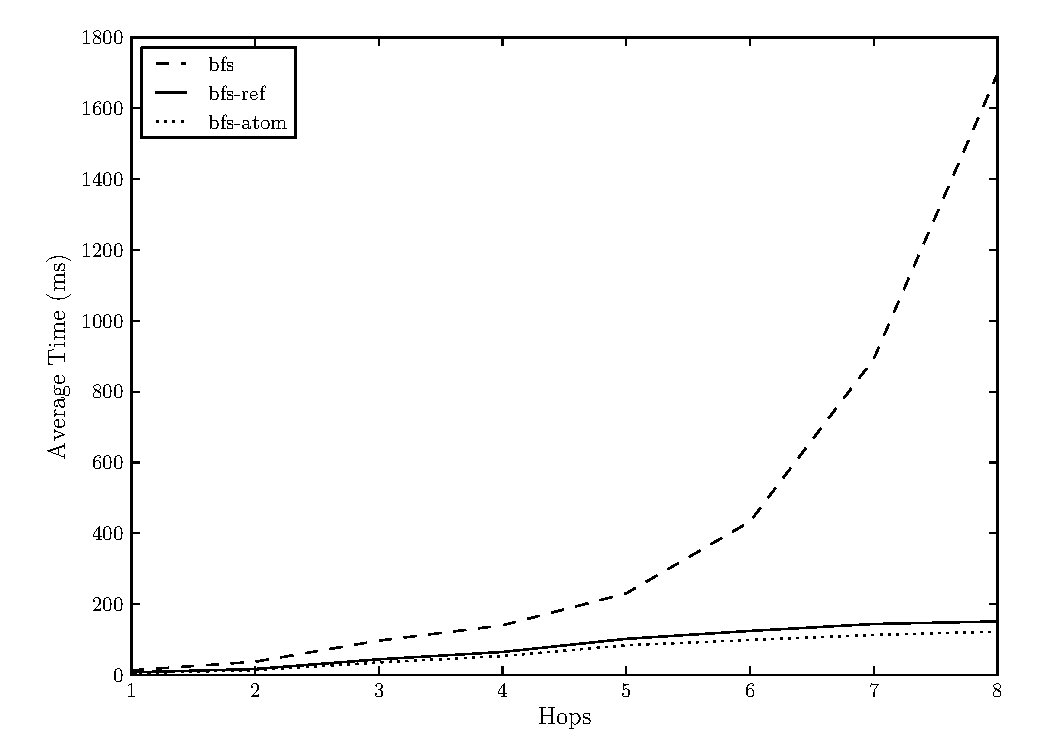
\includegraphics[scale=0.85]{growth}
			\caption{Comparison between single threaded and concurrent graph search}
			\label{fig:perf-growth}
		\end{figure}
	
	\chapter{Conclusion}
		\cite{rob-java-bench-08}
	
	% appendix
	\appendix
	
	\singlespacing
	
	% !TEX root = Thesis.tex
	
\chapter{Source Code}
	Each namespace in the code is divided into sections in the thesis document.
	  
	\section{molly}
		\subsection{molly.core}
			The core namespace is responsible for determining, provided a series of command line arguments, which action to take.  This namespace is invoked as the main class when the \gls{jar} is executed.
			
			\inputpygments{clj}{../../src/clj/molly/core.clj}
	
	\clearpage
	\section{molly.conf}
		\subsection{molly.conf.config}
			This namespace contains helper functions for loading part of the system configuration.  It also provides a protocol, \texttt{IConfig}, that is used to define the rest of the system configuration.
			
			\inputpygments{clj}{../../src/clj/molly/conf/config.clj}
		  
		\clearpage
		\subsection{molly.conf.mycampus}
			This is a sample configuration.  It defines the entities and relations in the mycampus dataset.
			
			\inputpygments{clj}{../../src/clj/molly/conf/mycampus.clj}
	
	\clearpage
	\section{molly.datatypes}
		There are several datatypes used in the system.
		\subsection{molly.datatypes.database}
			A protocol and concrete datatype are defined which provide access to a relational database.  Users creating an instance of this datatype are able to execute arbitrary queries, and must provide a function to apply to every tuple that is returned.
			
			\inputpygments{clj}{../../src/clj/molly/datatypes/database.clj}
		
		\clearpage
		\subsection{molly.datatypes.entity}
			One of the most important namespaces represents entities.  It includes functions to transform a named tuple from a database row into the internal representation as well as into documents.  It also includes auxiliary functions to produce a unique identifier.
			
			\inputpygments{clj}{../../src/clj/molly/datatypes/entity.clj}
		
		\clearpage
		\subsection{molly.datatypes.schema}
			The final datatype represents a schema.  These schemas contain a function that is used to execute the necessary \gls{sql} statements to retrieve all data from the relational database and place it in the full-text search index.
			
			Several of these schema datatypes are joined together in a configuration to produce a schema graph.
			
			\inputpygments{clj}{../../src/clj/molly/datatypes/schema.clj}
	
	\clearpage
	\section{molly.index}
		\subsection{molly.index.build}
			This namespace contains the function used to build the full-text search database.  It takes advantage of the fact that each schema knows how to construct its own documents.  The function simply iterates through every schema in the configuration, instructing them to index themselves.
			
			\inputpygments{clj}{../../src/clj/molly/index/build.clj}
	
	\clearpage
	\section{molly.util}
		\subsection{molly.util.nlp}
			The \texttt{q-gram} function computes the \(q\)-gram of a string.  Optionally a value for \(q\) and the padding character can be specified.
			
			\inputpygments{clj}{../../src/clj/molly/util/nlp.clj}
	
	\clearpage
	\section{molly.search}
		\subsection{molly.search.lucene}
			This namespace contains functions for interfacing with the Lucene library.  These functions include opening, adding documents, searching, and closing indices.
			
			\inputpygments{clj}{../../src/clj/molly/search/lucene.clj}
		
		\clearpage
		\subsection{molly.search.query\_builder}
			Phrase queries are used as they require each term in the phrase to be in a specific order.  This permits more accurate results as course titles and other items are in a specific order.
			
			These queries may be combined, creating a boolean query.
			
			\inputpygments{clj}{../../src/clj/molly/search/query_builder.clj}
	
	\clearpage
	\section{molly.server}
		This namespace contains functionality to expose the system functionality to clients over \gls{http}.
		
		\subsection{molly.server.core}
			\inputpygments{clj}{../../src/clj/molly/server/core.clj}
		
		\clearpage
		\subsection{molly.server.remotes}
			Rather than handle serialization over \gls{http} manually, the system uses the Shoreleave library\footnote{\url{https://github.com/shoreleave/shoreleave-remote}}.  It permits ClojureScript clients to transparently call functions exposed on the server.  The \texttt{defremote} macro is used to expose these functions.
			
			\inputpygments{clj}{../../src/clj/molly/server/remotes.clj}
		
		\clearpage
		\subsection{molly.server.search}
			This namespace provides the ``glue'' between the system and \gls{http} interface.
			
			\inputpygments{clj}{../../src/clj/molly/server/search.clj}
	
	\clearpage
	\section{molly.algo}
		\subsection{molly.algo.common}
			\inputpygments{clj}{../../src/clj/molly/algo/common.clj}
		
		\clearpage
		\subsection{molly.algo.bfs}
			\inputpygments{clj}{../../src/clj/molly/algo/bfs.clj}
		
		\clearpage
		\subsection{molly.algo.bfs\_atom}
			\inputpygments{clj}{../../src/clj/molly/algo/bfs_atom.clj}
		
		\clearpage
		\subsection{molly.algo.bfs\_ref}
			\inputpygments{clj}{../../src/clj/molly/algo/bfs_ref.clj}
	
	\clearpage
	\section{molly.bench}
		\subsection{molly.bench.benchmark}
			\inputpygments{clj}{../../src/clj/molly/bench/benchmark.clj}
	
	\printbibliography
	
	\todos
\end{document}
